\documentclass{article}
\usepackage{hyperref}
\usepackage{multirow}
\usepackage{graphicx}
\graphicspath{ {./images/} }

\title{Kaggle Competitions with Spark}
\author{Thomas Goethals, Kevin Cool, Miquel Vande Velde}
\begin{document}
	\maketitle
	\section{Digit Recognition}
	\subsection{Description}
		The kaggle competition entered was one to recognise hand written digits: \url{https://www.kaggle.com/competitions/digit-recognizer}. The most successfull machine learning models in this competition were convolutional neural networks (using the keras package). However, other classification algorithms seemed to be performing very good as well. \href{https://www.kaggle.com/code/alphaghostusmc/mnist-randomforest}{This} notebook achieved a (self reported) accuracy of 96\% using a random forest classifier. Note that this accuracy was achieved on a test split of the training data, not the actual competition test data.
	\subsection{Comparing Spark with Notebook entries}
	\subsubsection{Models}
	As mentioned above, the winning algorithm in Kaggle was, not surprisingly, a convolutional neural network, which is famous for image recognition. This model is not available in spark. However other classification techniques are also achieving high scores, with accuracies of more than 95\%. 
	As shown in the results below, I was able to reproduce these figures with spark.
	Using the default values offered in spark I only achieved an out of sample accuracy of 83\%. Comparing the documentation of scikit and spark I noticed some differences in default configuration. In scikit learn the max depth of the trees is indefinite as opposed to 5 in spark and the amount of trees is 100, compared to 20 in spark. To find the best configuration I made use of spark's CrossValidator to tune these hyperparameters and reached an accuracy of 96\%. The model achieved almost the same accuracy on submission see image below, indicating that it was not just overfitting.
	\subsubsection{Feature Engineering}
	In this competition feature engineering was not required to achieve high scoring results.
	
	\subsection{Results}
		\begin{tabular}{ |p{3cm}||p{3cm}| }
			\hline
			\multicolumn{2}{|c|}{Random Forest} \\
			\hline
			Algorithm& Accuracy\\
			\hline
			Kagel entry	& 	96\%\\
			Spark default&   83\%\\
			More trees &	93\%\\
			More depth &	96\%\\
			\hline
		\end{tabular}
		\begin{figure}[h]
			\centering
			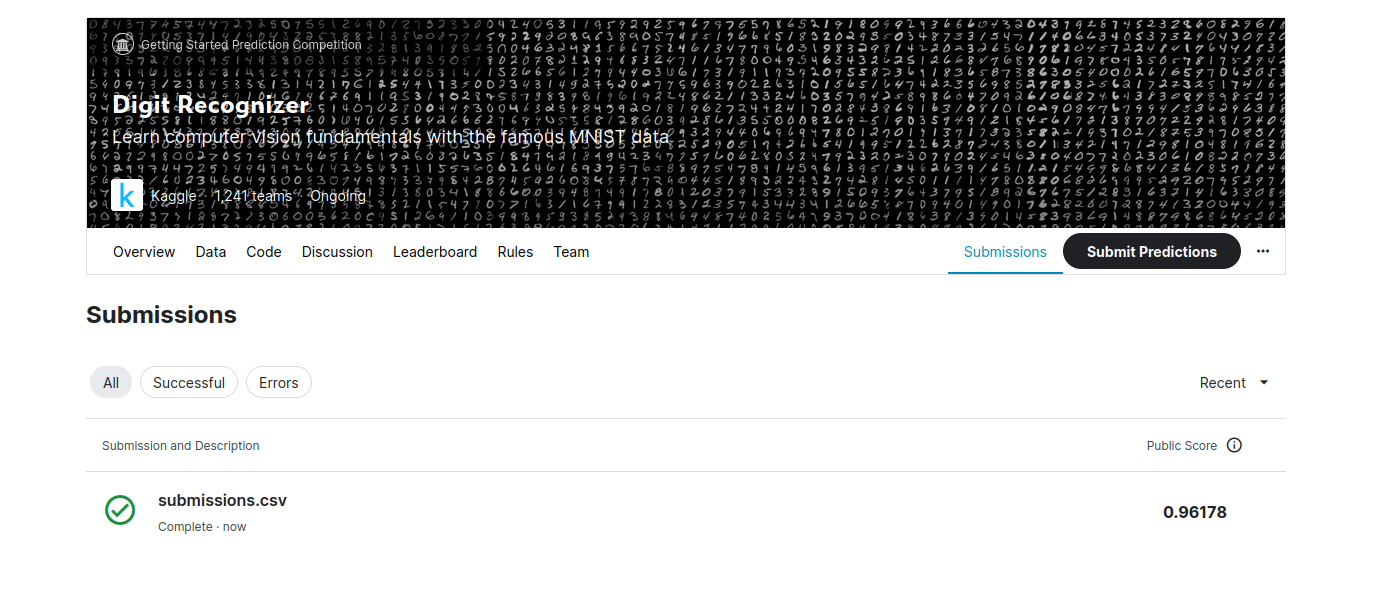
\includegraphics[scale=0.30]{submission_random_forest}
			\caption{Random forest submission results.}
		\end{figure}
	\section{Second Kaggle Competition}
	\section{Third Kaggle Competition}
\end{document}